\documentclass[border=5pt]{standalone}

\usepackage{tikz,pgfplots}
\begin{document}
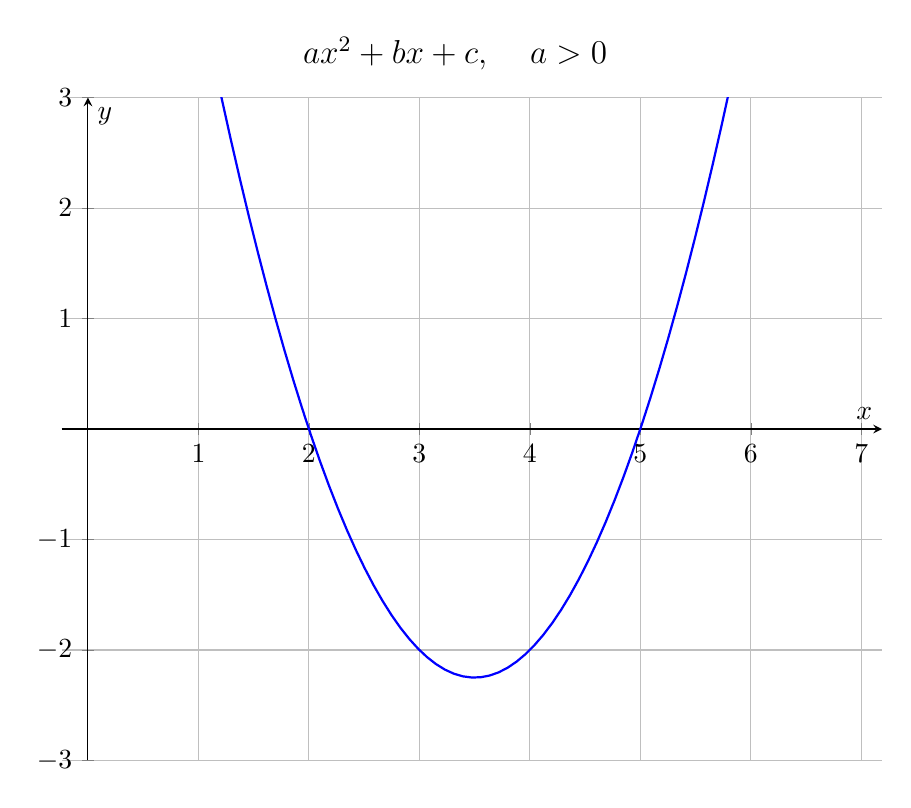
\begin{tikzpicture}
\begin{axis}[
    axis y line=center,
    axis x line=middle,
    axis equal,
    grid=both,
    domain=0:8,
    samples=100,
    ymin=-3,
    ymax=3,
    xlabel=$x$,
    ylabel=$y$,
    width=12cm,
    height=10cm,
]
\addplot[sharp plot,blue,thick] {(x-2)*(x-5)} ;
\end{axis}
\node[above,font=\large\bfseries] at (current bounding box.north) {$ax^2+bx+c,\quad a>0$};
\end{tikzpicture}
\end{document}